\chapter{Uniform Encoding and Applications}\chlabel{uel}
The partial prefix-free codes designed and studied in this chapter
will all be denoted $C : \Omega \to \{0, 1\}^* \cup \{\bot\}$, where
$\Omega$ is to be understood from context.

\section{The Uniform Encoding Lemma}

\begin{lem}\lemlabel{uel}
  Let $C : \Omega \to \{0, 1\}^* \cup \{\bot\}$ be a partial
  prefix-free code. Let $x \in \Omega$ be chosen uniformly at
  random. Then, for any $s \geq 0$,
  \[\Pr\left[\,|C(x)| \leq \log |\Omega| - s\,\right]
  \leq 2^{-s}.\]
\end{lem}
\begin{proof}
  Recall that we chose $|\bot| = \infty$, so if
  $C(x) \leq \log |\Omega| - s$, then $C(x)$ is defined.
  %Since $C$ is
  %bijective, then uniform selection of $x \in \Omega$ implies uniform
  %selection of $C(x)$ among all codewords of $C$.
  Let $k = \log |\Omega| - s$. Since $C$ has $|\Omega|$ codewords, and
  at most $2^k$ of those have length at most $k$, then the probability
  that $C(x)$ has length at most $k$ is at most
  \[\frac{2^{k}}{|\Omega|} = \frac{2^{\log |\Omega| - s}}{|\Omega|} =
  \frac{1}{2^s}. \qedhere\]
\end{proof}

This lower tail inequality is analogous to \thmref{incompressibility}
and is similarly crucial in proving results through encoding. The
approach is virtually the same as that described in
\secref{k-complexity}---only now, the length of an effective
description of an object is the length of its corresponding
prefix-free code.

For example usage of \lemref{uel}, see the proof of
\propref{binary-runs}.

\section{Permutations and Binary Search Trees}

\begin{defn}
  %A \emph{permutation} of size $n$ is a bijection
  %$\sigma : \{1, \ldots, n\} \to \{1, \ldots, n\}$, sometimes denoted
  %\[\sigma = (\sigma(1), \ldots, \sigma(n)).\]
  %The number of distinct permutations of size $n$ is $n!$.
  %is a sequence of $n$
  A \emph{permutation} $\sigma$ of size $n$ is a sequence of $n$
  distinct integers, sometimes denoted
  \[\sigma = (\sigma(1), \ldots, \sigma(n)).\]
  Except when explicitly stated, we will assume that the set of
  integers involved in a permutation of size $n$ is precisely
  $\{1, \ldots, n\}$. The number of such permutations is $n!$.
\end{defn}

%\subsection{Longest Ascending Run}
%
%\begin{defn}
%  For a permutation $\sigma$ of size $n$, an \emph{ascending run} of
%  length $k$ is a tuple
%  $(\sigma(i_1), \sigma(i_2), \ldots, \sigma(i_k))$ where
%  $1 \leq i_1 < \cdots < i_k \leq n$ and
%  $\sigma(i_1) < \cdots < \sigma(i_k)$.
%\end{defn}
%
%The length of the longest ascending run in a random permutation has
%been well-studied. Logan and Shepp~\cite{logan.shepp:runs} together
%with Vershik and Kerov~\cite{vershik.kerov:runs} are the first who
%established that the expected length of the longest ascending run in a
%random permutation is asymptotically $2\sqrt{n}$. Several new original
%proofs of this fact have appeared more recently; accordingly, we
%present an encoding argument to study this problem.
%
%\begin{thm}
%  Let $\sigma$ be a uniformly random permutation of size $n$. Then,
%  the longest ascending run in $\sigma$ has length at most
%  $(e + o(1))\sqrt{n}$ with probability $1 - O(1/n)$.
%\end{thm}
%\begin{proof}
%  We encode a permutation $\sigma$, which is chosen uniformly at
%  random from a set of size $n!$.
%
%  Suppose that $\sigma$ has an ascending run of length $t$. We encode
%  $\sigma$ by providing the set of values in this run; then the
%  indices in which they appear; and finally, the rest of the
%  permutation. Therefore,
%  \begin{align}
%    |C(\sigma)| &\leq 2 \log {n \choose t} + \log (n - t)! + O(1) \notag \\
%                &= \log n! + 2 \log {n \choose t} - \sum_{0 \leq i < t} \log (n - i) + O(1) \notag \\
%                &\leq \log n! + 2 t \log n - 2t \log t + 2t \log e - \sum_{0 \leq i < t} \log (n - i) + O(1) \tag{by \eqref{binom-code-loose}} \\
%                &\leq \log n! + t \log n - 2t \log t + 2t \log e + t \log \left(1 + \frac{t}{n - t} \right) + O(1) \notag \\
%                &\leq \log n! - 2t \log (t/e\sqrt{n}) + \frac{t^2}{n - t} \log e +
%                  O(1), \eqlabel{ascending-run-part}
%  \end{align}
%  where this last inequality follows since $1 + x \leq e^x$ for all $x
%  \in \R$. Choose $t = \ceil{e\sqrt{n} + (1/2)\ln n}$. Note that $t
%  \leq n/2$ for sufficiently large $n$, so $n - t \geq n/2$ and
%  \[
%  \frac{t^2}{n - t} \leq 2\left(e + \frac{\ln n}{2\sqrt{n}} + O(1/\sqrt{n})\right)^2
%  = O(1),
%  \]
%  so \eqref{ascending-run-part} becomes
%  \begin{align*}
%    |C(\sigma)| &\leq \log n! - 2 \left(e\sqrt{n} + \frac{1}{2}\ln n\right) \log \left(1 + \frac{\ln n}{2e\sqrt{n}}\right) + O(1) \\
%                &\leq \log n! - 2 e \sqrt{n}\log \left(1 + \frac{\ln
%                  n}{2e\sqrt{n}}\right) + O(1).
%  \end{align*}
%  Applying \lemref{uel}, we obtain that $\sigma$ has an ascending run
%  of length $e \sqrt{n} + (1/2)\ln n$ with probability
%  \[O\left(\left(1 + \frac{\ln
%        n}{2e\sqrt{n}}\right)^{-2e\sqrt{n}}\right) = O(e^{-\ln
%    n}) = O(1/n). \qedhere\]
%\end{proof}


\subsection{Records}\seclabel{records}

\begin{defn}
  A \emph{(max) record} in a permutation $\sigma$ of size $n$ is some
  value $\sigma(i)$ with $1 \leq i \leq n$ such that $\sigma(i) =
  \max\{\sigma(1), \ldots, \sigma(i)\}$.
\end{defn}

It is easy to see that the probability that $\sigma(i)$ is a record is
exactly $1/i$, so the expected number of records in a uniformly random
permutation is
\[H_n = \sum_{i = 1}^n \frac{1}{i} = \ln n + O(1),\] the
$n$\textsuperscript{th} harmonic number. It is harder to establish
concentration with non-negligible probability. To do this, one first
needs to show the independence of certain random variables, which
quickly becomes tedious. We instead give an encoding argument to show
concentration of the number of records inspired by a technique used by
Lucier \emph{et al.}~to study the height of random binary search
trees~\cite{lucier.jiang.li:quicksort}.

First, we describe an incremental and recursive manner of encoding a
permutation $\sigma$: begin by providing the first value of the
permutation $\sigma(1)$; followed by the indices of the permutation
for which $\sigma$ takes on a value strictly smaller than $\sigma(1)$,
including an explicit encoding of the induced permutation on the
elements at those indices; and a recursive encoding of the permutation
induced on the elements strictly larger than $\sigma(1)$.

If $\sigma$ contains $k$ elements strictly smaller than $\sigma(1)$,
then the size $S$ of the decision space above satisfies the recurrence
\[S(n) = n \binom{n - 1}{k} k! \cdot S(n - k - 1),\]
with $S(0) = 1$ and $S(1) = 1$. This solves to $S(n) = n!$, so the
encoding described above is no better than a fixed-length encoding for
$\sigma$.

We can readily modify the encoding above to obtain a result about the
concentration of records in a random permutation.

\begin{thm}\thmlabel{records}
  A uniformly random permutation of size $n$ has at least $c \log n$
  records with probability at most
  \[2^{-c (1 - H(1/c)) \log n + O(\log \log n)},\]
  for $c > 2$.
\end{thm}
\begin{proof}
  We encode a permutation $\sigma$ chosen uniformly at random from a
  set of size $n!$.

  Suppose that $\sigma$ has $t \geq c\log n$ records $r_1 < r_2 <
  \cdots < r_t$, for some fixed $c > 2$. First, give a bit string $x =
  x_1 \cdots x_t \in \{0, 1\}^t$, where $x_i = 0$ if and only if $r_i$
  lies in the first half of the interval $[r_{i - 1}, n]$. It follows
  that $n_1(x) \leq \log n$.
%Let $d_i$ denote the number of values of $\sigma$
  %which are greater than $r_i$. If $x_i = 1$, then
  %\[d_{i + 1} \leq (1/2) d_i,\]
  %and therefore,
  %\[1 \leq (1/2)^{n_1(x)} n \iff n_1(x) \leq \log n.\]
  In other words, $x$ is a sparse bit string, and $n_1(x)/t \leq 1/c$.

  To begin our encoding of $\sigma$, we encode the bit string $x$ by
  giving the set of $n_1(x)$ ones in $x$; followed by the incremental
  recursive encoding of $\sigma$ from earlier. In this case, our
  knowledge of the value of $x_i$ halves the size of the space of
  options for encoding the record $r_i$. In other words, our knowledge
  of $x$ allows us to encode each record using roughly one less bit
  per record. More precisely, since the encoding from above recurses
  $t$ times on decreasing values $n_1 > \cdots > n_t$, then the number
  of bits spent encoding records is at most
  \begin{align*}
    \sum_{i = 1}^t \log \lceil n_i/2 \rceil &\leq \sum_{i = 1}^t \log (n_i/2 + 1)
                                              \leq \sum_{i = 1}^t \log (n_i/2) + \sum_{i = 1}^t O(1/n_i) \\
                                            &\leq \sum_{i = 1}^t \log (n_i/2) + H_t = \sum_{i = 1}^t \log n_i - t + O(\log \log n).
  \end{align*}
  Thus, by \lemref{incremental-code}, the total length of the code is
  \begin{align*}
    |C(\sigma)| &\leq \binom{t}{n_1(x)} + \log n! - t + O(\log \log n) \\
                &\leq \log n! - t (1 - H(n_1(x)/t)) + O(\log \log n) \tag{by \eqref{binom-code-tight}}\\
                &\leq \log n! - c (1 - H(1/c))\log n + O(\log \log n).
  \end{align*}
  This last inequality holds since the function $x H(a/x)$ has
  derivative
  \[
  \frac{d}{d x} x H(a/x) = \log \frac{1}{1 - a/x},
  \]
  which is positive as long as $0 < a/x < 1$, and so increases as a
  function of $x$. Applying \lemref{uel}, we obtain the desired
  result.
  %has at most $c \log n$ records with probability $1 - O(1/n)$ for
  %$c \geq 2$ satisfying
  %\[c (1 - H(1/c)) \geq 1.\]
  %A computer-aided calculation shows that $c = 4.40349...$ is the
  %minimal solution to this inequality.
\end{proof}

\subsection{Tree Height}\seclabel{height}

Every permutation $\sigma$ determines a binary search tree
$\text{BST}(\sigma)$ created through the sequential insertion of the
keys $\sigma(1), \ldots, \sigma(n)$. Specifically, if $\sigma_L$
(respectively, $\sigma_R$) denotes the permutation of elements
strictly smaller (respectively, strictly larger) than $\sigma(1)$,
then $\text{BST}(\sigma)$ has $\sigma(1)$ as its root, with
$\text{BST}(\sigma_L)$ and $\text{BST}(\sigma_R)$ as left and right
subtrees. For any $\sigma$, the value $\sigma(1)$ is called its pivot.

Lucier \emph{et al.}~\cite{lucier.jiang.li:quicksort} use an encoding
argument via Kolmogorov complexity to study the height of
$\text{BST}(\sigma)$. They show that for a uniformly chosen
permutation $\sigma$, the tree $\text{BST}(\sigma)$ has height at most
$c \log n$ with probability $1 - O(1/n)$ for $c = 15.498...$; we can
extend our result on records to obtain a tighter result.

For a node $u$, let $s(u)$ denote the number of nodes in the tree
rooted at $u$. Then, $u$ is called balanced if $s(u_L), s(u_R) >
s(u)/4$, where $u_L$ and $u_R$ are the left and right subtrees of $u$
respectively. In other words, a node is said to be balanced if it
occurs in the middle half of its subrange. See
\figref{binary-insertion-tree}.

\begin{figure}
  \centering
  \begin{forest}
    [
    [$10$, for tree={draw,circle,text height=1.5ex,text depth=.25ex,l sep=0.5cm,s sep=1cm,inner sep=0.1cm}
      [$3$
        [$1$
          [,.phantom]
          [$2$]
        ]
        [$7$
          [$5$
            [$4$]
            [$6$]
          ]
          [$9$
            [$8$]
            [,.phantom]
          ]
        ]
      ]
      [$12$
        [$11$]
        [$13$]
      ]
    ]
    ]
  \end{forest}

  \caption{The tree $\text{BST}(\sigma)$, where $\sigma = (10, 12, 3,
    7, 1, 2, 5, 11, 9, 6, 13, 4, 8)$. $\sigma$ has records $10, 12,
    13$. The nodes $5, 7, 12$ are balanced.}
  \figlabel{binary-insertion-tree}
\end{figure}

\begin{thm}\thmlabel{bst-height}
  Let $\sigma$ be a uniformly random permutation of size $n$. Then,
  $\text{BST}(\sigma)$ has height $O(\log n)$ with high probability.
\end{thm}
\begin{proof}
  Suppose that the tree $\text{BST}(\sigma)$ has a rooted path $Y =
  y_1 \cdots y_t$ of length $t \geq c \log n$ for some fixed $c >
  2/\log (4/3)$.

  Our encoding for $\sigma$ has two parts. The first part includes an
  encoding of the value $y_t$, and a bit string $x = x_1 \cdots x_t$,
  where $x_i = 1$ if and only if $y_i$ is balanced. From our
  definition, if $y_i$ is balanced, then
  \[s(y_{i + 1}) \leq (3/4) s(y_i),\]
  and since $n_1(x)$ counts the number of balanced nodes along $Y$,
  then
  \[1 \leq (3/4)^{n_1(x)} n \iff n_1(x) \leq \log_{4/3} n.\]

  The second part of our encoding is recursive: first, encode the
  value of the root $r$ using $\log \lceil n/2 \rceil$ bits. If the
  path $Y$ goes to the left of $r$, then specify the values in the
  right subtree of $r$, including an explicit encoding of the
  permutation induced by these values; and recursively encode the
  permutation of values in the left subtree of $r$. If, instead, $Y$
  goes to the right of $r$, we proceed symmetrically.
 
  The first part of our encoding uses at most
  \[\log n + t H\left(\frac{n_1(x)}{t}\right)\]
  bits. The same analysis as performed in \thmref{records} shows that
  the second part of our encoding has length at most
  \[\log n! - t + O(\log \log n).\]
  Applying \lemref{uel}, we see that $\text{BST}(\sigma)$ has height
  at most $c \log n$ with probability $1 - O(1/n)$ for
  $c > 2/\log (4/3)$ satisfying
  \[c \left(1 - H\left(\frac{1}{c \log (4/3)}\right)\right) > 1,\]
  and a computer-aided calculation shows that $c = 8.12669...$ is the
  minimal solution to this inequality.
\end{proof}

\begin{rem}
  Devroye~\cite{devroye:records} shows how the length of the path to
  the key $i$ in $\text{BST}(\sigma)$ relates to the number of records
  in $\sigma$. Specifically, he notes that the number of records in
  $\sigma$ is the number of nodes along the rightmost path in
  $\text{BST}(\sigma)$. Since the height of a tree is the length of
  its longest root-to-leaf path, we obtain as a corollary that the
  number of records in a uniformly random permutation is $O(\log n)$
  with high probability; the result from \thmref{records} only
  improves upon the implied constant.
\end{rem}

%\Pr[|N - EN| > \eps EN] \leq 1/(\eps^2 H_n)

\begin{comment}
\begin{thm}[Lucier \emph{et al.}]\thmlabel{bst-height}
  Let $\sigma$ be a uniformly random permutation of size $n$. Then,
  $\text{BST}(\sigma)$ has height $O(\log n)$ with high probability.
\end{thm}
\begin{proof}
  We encode $\sigma$, which is chosen uniformly at random from a set
  of size $n!$.

  Suppose that $\text{BST}(\sigma)$ has a root-to-leaf path $x$ of
  length $t \geq c \log n$ for some fixed constant $c > 0$, with nodes
  $x_1, \ldots, x_{t + 1}$. Let $y = y_1 \cdots y_t \in \{0, 1\}^t$ be
  such that $y_i = 1$ if and only if $x_i$ is balanced. From our
  definition, if $x_i$ is balanced, then
  \[s(x_{i + 1}) \leq (3/4) s(x_i),\]
  and since $n_1(y)$ counts the number of balanced nodes along $x$,
  then
  \[1 \leq (3/4)^{n_1(y)} n \iff n_1(y) \leq \log_{4/3} n.\]
  Also, let $z = z_1 \cdots z_t \in \{0, 1\}^t$ be such that $z_i = 1$
  if and only if $s(z_i) < s(z_i')$, or if $s(z_i) = s(z_i')$ and
  $z_i$ is the left child of $z_{i - 1}$, where $z_i'$ is the sibling
  of $z_i$, \emph{i.e.} if $z_i$ is the right child of its parent,
  then $z_i'$ is the left child of $z_{i - 1}$, and vice versa. It is
  clear that
  \[s(z_i) \leq (1/2) s(z_{i - 1}),\]
  so $n_1(z) \leq \log n$.

  The code first consists an encoding for the bit string $yz$---since
  \[n_1(yz) \leq \left(\frac{1}{\log 4/3} + 1\right) \log n,\]
  as we showed above, and $|yz| = 2t \geq 2c \log n$, we make use of
  \lemref{bitstring-compression}. The rest of the code is a recursive
  encoding of $\sigma$ according to the structure of
  $\text{BST}(\sigma)$. We begin by encoding the value of $\sigma(1)$;
  if $\sigma(1)$ is part of the path $x$, we restrict its choice of
  options to only balanced or unbalanced nodes along the path,
  according to the information given previously; then, we give the
  values of the elements in $\sigma_L$; and finally, the recursive
  descriptions of the permutations $\sigma_L$ and $\sigma_R$.

  If the space of choices for each pivot were unrestricted, this
  decision space would have size
  $n {n - 1 \choose \ell} \ell! (n - \ell - 1)! = n!$. Since half of
  the values in any given range are unbalanced, then each node along
  $x$ decreases the size of the decision space by a factor of $2$. So,
  by \lemref{incremental-code}, the total code has length at most
  \begin{align*}
    b & \leq 2t H(n_1(yz)/2t) + \log (n!/2^t) + O(\log t) \\
      & \leq 2c \log n H\left(\frac{1 + 1/\log (4/3)}{2c}\right) + \log n! - t + O(\log \log n) \\
      & \leq \log n! - c \log n\left(1 - 2 H\left(\frac{1 + 1/\log (4/3)}{2c}\right)\right) + O(\log \log n).
  \end{align*}
  For sufficiently large $c$, applying \lemref{uel}, we obtain that
  $\text{BST}(\sigma)$ has height $O(\log n)$ with probability
  $1 - O(1/n)$.
\end{proof}

\begin{rem}
  Devroye~\cite{devroye:records} shows how the length of the path to
  the key $i$ in $\text{BST}(\sigma)$ relates to the number of records
  in $\sigma$. In particular, the number of nodes along the rightmost
  path in $\text{BST}(\sigma)$ is the number of records in
  $\sigma$. Since the height of a tree is the length of its longest
  root-to-leaf path, then \thmref{bst-height} implies that the number
  of records in a uniformly random permutation is also $O(\log n)$
  with high probability.
\end{rem}
\end{comment}

\section{Hashing}

In this section, we tackle the problem of implementing the hash table
data type. For an introduction to the study of data structures in
general and including hash tables, see the book by
Morin~\cite{morin:open}. A hash table supports the following
operations:
\begin{itemize}
\item $\textsc{Insert}(x)$: inserts $x$ into the hash table;
\item $\textsc{Delete}(x)$: deletes $x$ from the hash table;
\item $\textsc{Search}(x)$: determines whether or not $x$ is currently
  held in the hash table.
\end{itemize}

Many hash tables are implemented by storing elements in an array. As
such, to store $n$ elements from a set $\Omega$, we typically require
an array $A$ of size $m \geq n$, and some method of assigning array
positions to elements of $\Omega$. In each case, we will determine
these array indices using $\text{Uniform}(\{1, \ldots, m\})$ random
variables which we call \emph{hash functions}.

%Under the \emph{random probing assumption}, each element $x \in X$
%comes with an infinite sequence of iud variables
%$x^{(0)}, x^{(1)}, \ldots \in \{0, \ldots, m - 1\}$, called its
%\emph{probe sequence}, from which its array index can be deduced.

Any good hash table performs all operations in $O(1)$ expected
time. It can be shown, however, that it is impossible for a hash table
to achieve $O(1)$ worst-case time for all
operations~\cite{dietzfelbinger:perfecthashing}. We are thus concerned
with obtaining $O(1)$ expected time for all operations, and minimizing
the worst-case time of operations in hash table implementations.

%TALK ABOUT HASH SETS.
%
%TALK ABOUT UNIVERSAL HASH FUNCTIONS.
%
%TALK ABOUT WORST CASE VS AVERAGE CASE VS DETERMINISTIC VS EXPECTED
%TIME ETC.
%
%TALK ABOUT PREVIOUS RESULTS.

\subsection{Balls in Urns}\seclabel{balls-in-urns}

Our first look at hashing employs a simple solution. We are concerned
with hashing the set $\Omega = \{x_1, \ldots, x_n\}$ using a hash
function $h : \Omega \to \{1, \ldots, n\}$. In practice, each value of
$h$ points to one of $n$ lists, to which an element $x \in \Omega$ is
appended during insertion. This is an instance of \emph{hashing with
  chaining}. The worst case time of any operation is the maximum
number of potential hashing collisions, or the length of the longest
list.

It may be helpful to think of this scenario as modeled by balls and
urns: effectively, we throw $n$ balls into $n$ urns independently and
uniformly at random, and we are concerned with the maximum number of
balls in any urn. We call this the \emph{balls-in-urns} model hash
table.

\begin{thm}
  The cost of any operation in the balls-in-urns model hash table is
  $O(\log n/\log \log n)$ with probability $1 - O(1/n)$.
\end{thm}
\begin{proof}
  We identify the values of $h$ with lists. Since each $h(x_i)$ is
  independent and uniformly distributed in $\{1, \ldots, n\}$, then
  the sequence $h(\Omega) = (h(x_1), \ldots, h(x_n))$ is uniformly
  distributed in a set of size $n^n$, and so will be the subject of
  our encoding.

  Suppose that the list corresponding to $h(x_i)$ has $t$
  elements. Our encoding begins by specifying the value of $i$; then
  the set of $t$ elements contained in this list; and finally the
  positions of the remaining $n - t$ hashed elements. Our code then
  has length
  \begin{align*}
    |C(h(\Omega))| &\leq \log n + \log {n \choose t} + (n - t) \log n + O(1) \\
                   &\leq \log n + t \log n - t \log t + t \log e + (n - t)\log n + O(1) \tag{by \eqref{binom-code-loose}} \\
                   &= \log n^n + \log n - t \log (t/e) + O(1) \\
                   &\leq \log n^n - s,
  \end{align*}
  as long as $t$ satisfies $t\log(t/e) \geq \log n + s + O(1)$.
  Particularly, if we let $s = \log n$, then we can choose
  \[t = \Ceil{\frac{(2 + \eps)\log n}{\log \log n}}\]
  for any $\eps > 0$ and sufficiently large $n$. We finish by applying
  \lemref{uel}.
\end{proof}

\subsection{Linear Probing}

In a \emph{linear probing} hash table, we require that $m = cn$, for
some $c > 1$. We again hash the set $\Omega$ using a hash function $h
: \Omega \to \{1, \ldots, m\}$. In this case, $h$ points to array
indices in some array $A$. To insert $x$ into the hash table, we
insert it into the first empty spot among $A[h(x)], A[h(x) + 1],
A[h(x) + 2], \ldots$, where each array index is taken modulo
$m$. Since $m > n$, this is always possible.

A maximal consecutive sequence of occupied indices in $A$ is called a
\emph{block}. The running time of any operation in a linear probing
hash table is bounded by the size of the largest block. See
\figref{linearprobing} for an example execution of the above algorithm

\begin{figure}
  \centering
  %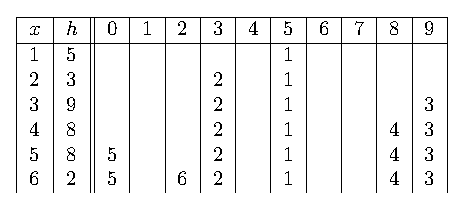
\includegraphics{linearprobing}
  %\begin{tabular}{|l|c||m{0.35cm}|p{0.35cm}|p{0.35cm}|p{0.35cm}|p{0.35cm}|p{0.35cm}|p{0.35cm}|p{0.35cm}|p{0.35cm}|p{0.35cm}|}\hline
  \begin{tabular}{|c|c|| *{10}{>{\centering\arraybackslash}p{0.35cm}|} } \hline
    $\#$ & $h(x)$ & $0$ & $1$ & $2$ & $3$ & $4$ & $5$ & $6$ & $7$ & $8$ & $9$ \\ \hline
    1 & $5$ & & & & & & $x_1$ & & & &\\
    2 & $3$ & & & & $x_2$ & & -- & & & &\\
    3 & $9$ & & & & -- & & -- & & & & $x_3$ \\
    4 & $8$ & & & & -- & & -- & & & $x_4$ & -- \\
    5 & $8$ & $x_5$ & & & -- & & -- & & & -- & -- \\
    6 & $2$ & -- & & $x_6$ & -- & & -- & & & -- & -- \\ \hline
  \end{tabular}
  \caption{A linear probing hash table undergoing the sequential
    insertion of elements $x_1, \ldots, x_6$. In the end, we see that
    $x_2$ and $x_6$ are in a block of size $2$; $x_1$ in a block of
    its own; and $x_3, x_4, x_5$ are in a block of size $3$.}
  \figlabel{linearprobing}
\end{figure}


\begin{lem}\lemlabel{linear-probing-lemma}
  Fix some $x \in \Omega$. In a linear probing hash table with
  $c > e$, the probability that $x$ belongs to a block of size at
  least $t$ satisfying
  \[
  t \log (c/e) - \log t \geq s + O(1)
  \]
  is at most $2^{-s}$.
\end{lem}
\begin{proof}
  Again, we encode the sequence $h(\Omega) = (h(x_1), \ldots, h(x_n))$
  which, for the same reason, is uniformly chosen from a set of size
  $m^n$.

  Suppose that $x$ belongs to a block of size $t$. Our encoding begins
  by providing the first index $i$ of the block containing $x$; then
  the set of the remaining $t - 1$ values in the block, which we call
  $y_1, \ldots, y_{t - 1}$; followed by enough information to decode
  the hash values $h(x), h(y_1), \ldots, h(y_{t-1})$; and finally, the
  hash values of the $n - t$ remaining elements of $\Omega$.

  Note that each of the values $h(x) - i, h(y_1) - i, \ldots,
  h(y_{t-1}) - i$ are within the range $0, 1, \ldots, t - 1$ modulo
  $m$, and so the hash values $h(x), h(y_1), \ldots, h(y_{t-1})$ can
  be encoded using $\lceil t \log t \rceil$ bits. From this
  discussion, we see that our code uses at most
  \begin{align*}
    |C(h(\Omega))| &\leq \log n + \log \binom{n}{t - 1} + t \log t + (n - t) \log m + O(1) \\
                   &\leq \log m^n + t\log n + (t - 1)\log e + \log t - t \log m + O(1) \tag{by \eqref{binom-code-loose}}\\
                   &\leq \log m^n + t\log (e/c) + \log t + O(1) \\
                   &\leq \log m^n - s
  \end{align*}
  bits, as long as $t$ is such that
  \[
  t \log (c/e) - \log t \geq s + O(1).
  \]
  The result follows from \lemref{uel}.
\end{proof}

%\begin{thm}\thmlabel{linear-probing-search}
%  Any operation in a linear probing hash table with $c > e$ takes time
%  at most $2 \log n + O(1)$ with probability $1 - O(1/n)$.
%\end{thm}
%\begin{proof}
%  Choose $s = 2 \log n$ in the previous lemma, so that any fixed $x
%  \in \Omega$ is contained in a block of size $2 \log n + O(1)$ with
%  probability $O(1/n^2)$. Then, by the union bound, no element is
%  contained in a block of size $2 \log n + O(1)$ with probability $1 -
%  O(1/n)$.
%  %A similar argument gives $O(1)$ expected time for any operation.
%\end{proof}

\begin{thm}
  A linear probing hash table with $c > e$ achieves $O(1)$ expected
  time for all operations.
\end{thm}
\begin{proof}
  Let $S$ denote the size of the largest block in such a hash
  table. From \lemref{linear-probing-lemma}, any fixed $x \in \Omega$
  is contained in a block of size at least $2s/\log (c/e) + d$ with
  probability at most $2^{-s}$, for some constant $d$. Then,
  \begin{align*}
    \E[S] &= \sum_{s = 1}^\infty \Pr[S \geq s] = \sum_{s = 1}^{d} \Pr[S \geq s] + \sum_{s = 1}^\infty \Pr[S \geq s + d] \\
          &\leq d + \sum_{s = 1}^\infty 2^{-s \log (c/e)/2} = d + \sum_{i = 1}^\infty \left(\frac{c}{e}\right)^{-s/2} = O(1). \qedhere
  \end{align*}
\end{proof}

%\subsection{Double Hashing}
%
%Encode the string $h_1(x_1) h_2(x_1) \ldots h_1(x_n)
%h_2(x_n)$. Suppose that some $x$ is contained in a block of size $t$.
%
%We encode $R$ by providing the first index $i$ of the block containing
%$x$; then the set of the remaining $t - 1$ values in the block which
%we call $y_1, \ldots, y_{t - 1}$; followed by enough information to
%decode the hash values $h(x), h(y_1), \ldots, h(y_{t-1})$; and
%finally, the hash values of the $n - t$ remaining elements of $X$.

\subsection{Cuckoo Hashing}\seclabel{cuckoo-hashing}

Cuckoo hashing is a simple and efficient hashing solution developed by
Pagh and Rodler which achieves $O(1)$ deterministic search
time~\cite{pagh.rodler:cuckoo}. The encoding arguments in this
section, due to P\u{a}tra\c{s}cu~\cite{patrascu:cuckoo}, neatly
establish some of the nice properties of cuckoo hashing.

The hash table consists of two arrays $A$ and $B$ of size $m = 2n$,
and two hash functions $h, g : \Omega \to \{1, \ldots, m\}$. To insert
an element $x$ into the hash table, we insert it into $A[h(x)]$; if
$A[h(x)]$ already contains an element $y$, we insert $y$ into
$B[g(y)]$; if $B[g(y)]$ already contains some element $z$, we insert
$z$ into $A[h(z)]$, etc. If an empty location is eventually found, the
algorithm terminates successfully. If a cycle is detected, then the
hash table is rebuilt using different hash functions. Any element $x$
either is held in $A[h(x)]$ or $B[g(x)]$, so we can search for $x$ in
$O(1)$ time.

To study the performance of insertion in cuckoo hashing, we study the
random bipartite \emph{cuckoo graph} $G$, where $V(G) = A \cup B$ with
bipartition $(A, B)$, with each vertex corresponding either to a
location in the array $A$ or $B$, and with edge multiset
$E(G) = \{(h(x), g(x)) : x \in \Omega\}$. Note that in this graph,
each edge corresponds to an element of $x$, and each vertex
corresponds to a position in the hash table.

An edge-simple path is a path which uses each edge at most once. Such
a path in this graph describes the potential motion of keys in a hash
table insertion. Thus, in bounding the length of edge-simple paths in
the cuckoo graph, we bound the worst case insertion time.
\begin{lem}\lemlabel{cuckoo-path-length}
  The cuckoo graph has an edge-simple path of length greater than
  $s + \log n + O(1)$ with probability at most $2^{-s}$.
\end{lem}
\begin{proof}
  We encode $G$ by presenting its set of edges. Since each endpoint of
  an edge is chosen independently and uniformly at random from a set
  of $n$ choices, then the set of all edges is chosen uniformly from a
  set of size $m^{2n}$.

  Suppose that some vertex $v$ is the endpoint of an edge-simple path
  of length $t$; such a path has $t + 1$ vertices and $t$ edges. In
  the encoding, we present the $t$ edges of the path in order; then,
  we indicate whether $v \in A$ or $v \in B$; and we give the $t + 1$
  vertices in order starting from $v$; and finally, the remaining
  $2n - 2t$ endpoints of edges of the graph. This code has length
  \begin{align*}
    |C(G)| &\leq t \log n + 1 + (t + 1) \log m + (2n - 2t) \log m + O(1)\\
           &= \log m^{2n} + t \log n - t \log m + \log m + O(1) \\
           &= \log m^{2n} - t + \log n + O(1) \tag{since $m = 2n$} \\
           &\leq \log m^{2n} - s
  \end{align*}
  for $t \geq s + \log n + O(1)$. We finish by applying \lemref{uel}.
\end{proof}

Choosing $s = \log n$ and applying the union bound, we see that
successful insertion takes time at most $2 \log n + O(1)$ with
probability $1 - O(1/n)$.

The cuckoo hashing insertion algorithm can fail if some subgraph of
the cuckoo graph contains more edges than vertices, since edges
correspond to keys, and vertices correspond to array locations.
\begin{lem}\lemlabel{cuckoo-failure}
  Fix some vertex $v \in A$. The probability that $v$ is part of a
  subgraph with more edges than vertices is $O(1/n^2)$.
\end{lem}
\begin{proof}
  Suppose that $v$ is part of a subgraph with more edges than
  vertices, and in particular a minimal such subgraph with $t + 1$
  edges and $t$ vertices. Such a subgraph appears exactly as in
  \figref{cuckoo-cycles}. For every such subgraph, there are two edges
  $e_1$ and $e_2$ whose removal disconnects the graph into two paths
  of length $t_1$ and $t_2$ starting from $v$, where
  $t_1 + t_2 = t - 1$.

  \begin{figure}
    \centering
    \begin{subfigure}[b]{0.3\textwidth}
      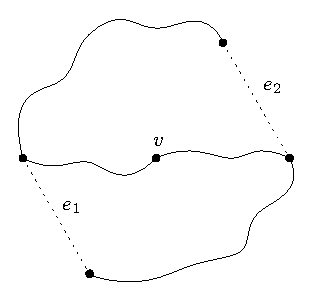
\includegraphics{cuckoo1}
      \caption{A cycle with a chord.}
    \end{subfigure}
    \quad\quad
    \begin{subfigure}[b]{0.6\textwidth}
      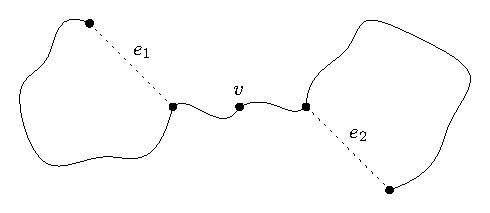
\includegraphics{cuckoo2}
      \caption{Two cycles connected by a path.}
    \end{subfigure}
    \caption{The potential minimal subgraphs of the cuckoo graph.}
    \figlabel{cuckoo-cycles}
  \end{figure}

  We encode $G$ by presenting Elias $\delta$-codes for the values of
  $t_1$ and $t_2$; then the edges of the above paths in order; then
  the vertices of the paths in order; and the edges $e_1$ and $e_2$;
  and finally the remaining $2n - 2(t + 1)$ endpoints of edges in the
  graph. Such a code has length
  \begin{align*}
    |C(G)| &\leq (t - 1)(\log n + \log m) + 2\log n + (2n - 2(t + 1))\log m + O(\log t) \\
           &= \log m^{2n} - 2\log m - t + O(\log t) \\
           &\leq \log m^{2n} - 2\log n + O(1).
  \end{align*}
  We finish by applying \lemref{uel}.
\end{proof}

From the union bound, we obtain the following:
\begin{cor}
  Cuckoo hashing succeeds upon insertion of $n$ elements with
  probability $1 - O(1/n)$.
\end{cor}

%\begin{rem}
%  TALK ABOUT HAVING MORE ARRAYS AND LOAD FACTOR AND SHIT LIKE THAT.
%\end{rem}

%Hashing analyzed through random bipartite
%graphs. \cite{pagh.rodler:cuckoo} \cite{patrascu:cuckoo}

\subsection{2-Choice Hashing}

We showed in \secref{balls-in-urns} that if $n$ balls are thrown
independently and uniformly at random into $n$ urns, then the maximum
number of balls in any urn is $O(\log n/\log \log n)$ with high
probability. In 2-choice hashing, another instance of hashing with
chaining, each ball is instead given a choice of two urns, and the urn
containing the fewer balls is preferred.

More specifically, we are given two hash functions $h, g : \Omega \to
\{1, \ldots, m\}$. Each value of $h$ and $g$ points to one of $m$
lists. The element $x \in \Omega$ is appended to the smaller list
between $h(x)$ and $g(x)$ during an insertion. The worst case search
time is at most the maximum number of hashing collisions, or the
length of the longest list.

Perhaps surprisingly, the simple change of having two choices instead
of only one results in an exponential improvement over the strategy of
\secref{balls-in-urns}. Indeed, 2-choice hashing was first studied by
Azar \emph{et al.}~\cite{azar:multiplechoice}, who showed that the
expected maximum size of an urn is $\log \log n + O(1)$. Our encoding
argument is based on V\"{o}cking's use of witness trees to analyze
2-choice hashing~\cite{vocking:witness}.

As in \secref{cuckoo-hashing}, we use random graphs to study the
performance of 2-choice hashing. Let $G$ be the random multigraph with
$V(G) = \{1, \ldots, m\}$, where $m = cn$ for some constant $c > e$,
and $E(G) = \{(h(x), g(x)) : x \in \Omega\}$.

%\begin{lem}
%  The multigraph $G$ has an edge-simple path of length greater than
%  $s + \log n + O(1)$ with probability at most $2^{-s}$.
%\end{lem}
%\begin{proof}
%  The proof is similar to that of \lemref{cuckoo-path-length}: again,
%  we encode the set of edges.
%
%  Suppose some vertex $v$ is the endpoint of an edge-simple path of
%  length $t$. We encode this path by presenting the $t$ edges in
%  order, including their orientation; then, the $t + 1$ vertices,
%  starting from $v$; and finally, the remaining $2n - 2t$ endpoints of
%  edges in the graph. Our code has length
%  \begin{align*}
%    |C(G)| &\leq t\log 2n + (t + 1)\log m + (2n - 2t)\log m + O(1) \\
%           &= 2n \log m + t \log 2n - t \log m + \log m + O(1) \\
%           &= \log m^{2n} + t \log \frac{2n}{m} + \log m + O(1) \\
%           &\leq \log m^{2n} + \log n - t + O(1) \\
%           &\leq \log m^{2n} - s,
%  \end{align*}
%  as long as $t \geq s + \log n + O(1)$, so apply \lemref{uel}.
%\end{proof}

\begin{lem}\lemlabel{two-choice-two-cycles}
  $G$ has a subgraph with more edges than vertices with probability
  $O(1/n)$.
\end{lem}
\begin{proof}
  The proof is similar to that of \lemref{cuckoo-failure}, with an
  additional application of the union bound. More specifically, we can
  encode $G$ by giving the same encoding as in
  \lemref{cuckoo-failure}, with an additional bit for each edge
  $(u, v)$ in the encoding, indicating whether $u = h(x)$ and
  $v = g(x)$, or $u = g(x)$ and $v = h(x)$. Our code thus has length
  \begin{align*}
    |C(G)| &\le (t - 1)(\log n + \log m) + 2 \log n + (2n - 2(t + 1))\log m + t + O(\log t) \\
           &= \log m^{2n} - 2 \log n - t \log c + t + O(\log t) \\
           &\le \log m^{2n} - 2 \log n + O(1) ,
  \end{align*}
  since $\log c > 1$.
\end{proof}


%\begin{lem}\lemlabel{two-choice-two-cycles}
%  With probability $1 - O(1/n)$, $G$ has no subgraph with more edges
%  than vertices.
%\end{lem}
%\begin{proof}
%  Again, the proof is similar to that of \lemref{cuckoo-failure}, with
%  an additional application of the union bound.
%\end{proof}

%\begin{lem}
%  Fix some $v \in \{1, \ldots, m\}$. The probability that $v$ belongs
%  to a component of $G$ of size at least $2 \log n$ is $O(1/n^2)$.
%\end{lem}
%\begin{proof}
%  Suppose $G$ has a connected component $C$ containing $v$ with
%  $t - 1$ edges and at most $t$ vertices. We encode the edge set of
%  $G$ by providing the set of vertices in a spanning tree of $C$
%  rooted at $v$; then the shape of this tree; and the labels of the
%  $t - 1$ edges encountered in an inorder traversal of this tree; and
%  finally the remaining $2(n - t + 1)$ endpoints of edges. By Cayley's
%  formula and since $G$ is a multigraph, there are at most $t^{t - 2}$
%  spanning trees of $G$ rooted at $v$. In total, our code has length
%  \begin{align*}
%    |C(G)| &\leq \log {m \choose t - 1} + (t - 2) \log t + (t - 1) \log n + 2 (n - t + 1) \log m + O(1) \\
%           &\leq 2n \log m - (t - 1) \log (c/e) - \log t + O(1) & \text{(by \eqref{binom-code-loose})} \\
%           &\leq \log m^{2n} - s,
%  \end{align*}
%  as long as $t$ is such that
%  \[t \log (c/e) + \log t \geq s + O(1).\]
%  In particular, if we choose $s = 2 \log n$, applying \lemref{uel}
%  tells us that $C$ has size at least $2 \log n$ with probability
%  $O(1/n^2)$.
%\end{proof}
%
%\begin{cor}\corlabel{two-choice-component-size}
%  With probability $1 - O(1/n)$, every component of $G$ has size at
%  most $2 \log n$.
%\end{cor}

\begin{lem}\lemlabel{two-choice-component-size}
  $G$ has a component of size at least $(2/\log(c/e))\log n + O(1)$
  with probability $O(1/n)$.
\end{lem}
\begin{proof}
  Suppose $G$ has a connected component $X$ with $t - 1$ edges and at
  most $t$ vertices. We encode the edge set of $G$ by providing the
  set of vertices in a spanning tree of $X$, and we choose to root
  this tree at the first vertex described in this set; then the shape
  of this tree; and the labels of the $t - 1$ edges encountered in an
  inorder traversal of this tree; and finally the remaining
  $2(n - t + 1)$ endpoints of edges. By Cayley's formula and since $G$
  is a multigraph, there are at most $t^{t - 2}$ rooted spanning trees
  of $G$. In total, our code has length
  \begin{align*}
    |C(G)| &\le \log \binom{m}{t} + (t - 2) \log t + (t - 1) \log n + 2 (n - t + 1) \log m + O(1) \\
           %&\le 2n \log m + t\log m + t\log e - 2\log t + (t-1)\log n - 2(t-1)\log m \tag{by \eqref{binom-code-loose}} \\
           &\le \log m^{2n} - t\log c + t\log e - 2\log t + \log n + O(1) \tag{by \eqref{binom-code-loose}} \\
           &\le \log m^{2n} - s ,
  \end{align*}
  as long as $t$ is such that
  \[t \log (c/e) + 2\log t \geq s + \log n + O(1) .\]
  In particular, if we choose $s = \log n$, applying \lemref{uel}
  tells us that $X$ has size at least $(2/\log (c/e))\log n + O(1)$
  with probability $O(1/n)$.
\end{proof}

Suppose that when $x$ is inserted, it is placed in a list with $t$
other elements. Then, we say that the age of $x$ is $a(x) = t$.
\begin{thm}
  The cost of any operation in 2-choice hashing is at most
  $\log \log n + O(1)$ with probability $1 - O(1/n)$.
\end{thm}
\begin{proof}
  Suppose that some element $x$ has $a(x) = t$. This leads to a binary
  \emph{witness tree} $T$ of height $t$ as follows.

  The root of $T$ is the element $x$. When $x$ was inserted into the
  hash table, it had to choose between the lists $h(x)$ and $g(x)$,
  both of which contained at least $t - 1$ elements; in particular,
  $h(x)$ has an element $x_h$ with $a(x_h) = t - 1$, and $g(x)$ has an
  element $x_g$ with $a(x_g) = t - 1$. The elements $x_h$ and $x_g$
  become left and right children of $x$ in $T$. The process continues
  recursively. If some element appears more than once on a level, we
  only recurse on its leftmost occurence.

  Note that each vertex of $T$ corresponds to the edge $(h(x), g(x))$
  of $G$. Moreover, the subgraph of $G$ induced by the edges
  $\{(h(x), g(x)) : x \in V(T)\}$ is connected.

  Suppose that some node appears more than once on a level of
  $T$. From above, this means that some component of $G$ has a
  cycle. If this happens twice, then $G$ has a subgraph with more
  edges than vertices. By \lemref{two-choice-two-cycles}, this happens
  with probability $O(1/n)$. If instead this happens at most once,
  then $T$ has at most one subtree removed, so $T$ has at least $2^t$
  nodes. If we choose $t = \ceil{\log \log n + d}$, then $T$ has at
  least $2^d \log n$ nodes, which we know from
  \lemref{two-choice-component-size} happens with probability $O(1/n)$
  for a sufficiently large choice of the constant $d$.
\end{proof}

%\subsection{Robin-Hood Hashing}
%Use random hypergraphs to encode the sequence:
%\begin{align*}
%  & h_1(x_1) \ldots h_k(x_1) \\
%  & h_1(x_2) \ldots h_k(x_2) \\
%  & \ldots \\
%  & h_1(x_n) \ldots h_k(x_n)
%\end{align*}

%Suppose that some element $x$ has $a(x) = t$. Then, this leads to a
%witness tree $T$ of height $t$ as follows.

%The root of $T$ is $x$. Let $x_1, \ldots, x_{t - 1}$ denote the
%sequence of elements currently held in
%$A[h_1(x)], \ldots, A[h_{t-1}(x)]$. When $x$ was moved from position
%$h_i(x)$, it competed with an older element $x_i'$ with
%$a(x_i') \geq i$, so $a(x_i) \geq a(x_i') \geq i$. Let $x$ have
%children $x_1, \ldots, x_{t - 1}$ in sequence, and recurse on them. If
%an element appears more than once, only recurse on its first
%occurence.

%Let $H = (V, E)$ be the hypergraph with vertices $\{1,\ldots, m\}$,
%and hyperedges $\{(h_1(x), \ldots, h_k(x)) : x \in X\}$. Each vertex
%of $T$ corresponds to a hyperedge in $H$, and the subhypergraph of $H$
%induced by these hyperedges is connected.

%\begin{thm}[Lavault]
%  The number of $k$-uniform hypertrees with $n$ edges is:
%  \[\frac{(n(k - 1))!}{n! (k - 1)!} (n(k - 1) - 1)^n\]
%\end{thm}

%Ahem... look at the bipartite incidence graph with bipartition
%$(V, E)$, such that $v \sim e$ if $h_i(v) \in e$ for some $i$.

%If some element $x \in X$ has $a(x) = t$, then

%--

%Consider the graph on vertex set $X^k$, with edges
%$(h_1(x), h_2(x)), (h_2(x), h_3(x)), \ldots, (h_{k-1}(x), h_k(x))$ for
%every $x \in X$. If there exists an $x \in X$ with $a(x) = t$, then
%the above witness tree gives a large connected component of the graph.
%\begin{align*}
%  \log {km \choose t - 1} + (t - 2)\log t 
%\end{align*}

\section{Bipartite Expanders}

Expanders are families of graphs which share some isoperimetric
quality, \emph{i.e.}~where subgraphs ``expand'' in their
neighbourhoods. These graphs have received much research attention,
and have been shown to have many applications in computer
science. See, for instance, the survey by Hoory, Linial, and
Wigderson~\cite{hoory.linial.ea:expander}.

Though expanders have proven to have fascinating qualities and be
remarkably useful, they have yet been difficult to construct. The
first proof of existence of expanders by Pinkser was
probabilistic~\cite{pinsker:on}. The first explicit construction,
given by Margulis, relied on advanced concepts in representation
theory~\cite{margulis:explicit}. Later constructions have become
simpler to analyze.

We offer an encoding argument to prove that a random bipartite graph
is an expander with high probability. Indeed, expanders are often
called ``pseudorandom'' graphs due to their many shared properties
with random graphs; one should expect, just as a random graph is
incompressible, so too are expanders.

There are many different notions of expansion. We will consider what
is commonly known as vertex expansion in bipartite graphs.
\begin{defn}
  Fix some $0 < \alpha \leq 1$. A bipartite graph $G$ with bipartition
  $(A, B)$ is a \emph{$(c, \alpha)$-expander} if
  \begin{align*}
    \min_{\substack{{A' \subseteq A}\\{|A'| \leq \alpha |A|}}} \frac{|N(A')|}{|A'|} \geq c,
  \end{align*}
  where $N(A') \subseteq B$ is the set of neighbours of $A'$ in $G$.
\end{defn}

Let $G$ be a random bipartite graph with bipartition $(A, B)$ where
$|A| = |B| = n$ and such that each vertex in $A$ is connected to three
vertices chosen uniformly at random in $B$.

\begin{thm}
  For some constant $\alpha > 0$, $G$ is a $(3/2, \alpha)$-expander
  with probability at least $1 - O(n^{-1/2})$.
\end{thm}
\begin{proof}
  Suppose that $G$ is not a $(3/2, \alpha)$-expander, so there exists
  some $A' \subseteq A$ where $|A'| \leq \alpha |A|$ and
  \[\frac{|N(A')|}{|A'|} < 3/2.\]
  We encode the graph $G$ by encoding its edge set, which is chosen
  uniformly at random from a set of size $n^{3n}$.

  Our encoding presents the value $k = |A'|$ using an Elias
  $\gamma$-code; then the sets $A'$ and $N(A')$, and the edges between
  them; and finally, the remaining edges of the graph. This costs
  \begin{align*}
    |C(G)| &\leq 2\log k + \log {n \choose k} + \log {n \choose 3k/2} + 3k \log (3k/2) + (3n - 3k)\log n + O(1) \nonumber\\
           &\leq \log n^{3n} - (k/2)\log n + (k/2)\log k + \beta k + 2 \log k + O(1) \tag{by \eqref{binom-code-loose}}\\
           &= \log n^{3n} - s(k) \nonumber
  \end{align*}
  bits, where $\beta = (3/2) \log (3/2) + (5/2) \log e$. Note that
  \[
  \frac{d^2}{d k^2} s(k) = \frac{4 - k}{2k^2} \log e ,
  \]
  so $s(k)$ is concave for all $k \geq 4$. Thus, $s(k)$ is minimized
  either when $k = 1, 2, 3, 4,$ or $k = \alpha n$. We have
  \begin{align*}
    s(1) &= (1/2)\log n + c_1, &  s(2) &= \log n + c_2, \\
    s(3) &= (3/2) \log n + c_3, & s(4) &= 2 \log n + c_4,
  \end{align*}
  for constants $c_1, c_2, c_3, c_4$. For $k=\alpha n$ we have
  \[
  s(\alpha n) = (\alpha n/2)\log \left(\frac{1}{2^{2 \beta}
      \alpha}\right) - 2 \log \alpha n + O(1)
  \]
  and $2^{-s(\alpha n)} = 2^{-\Omega(n)}$ for $\alpha < (1/2)^{2
    \beta}$. In each case, apply \lemref{uel}.
\end{proof}
